\section{Sewer interconnection}\label{se:sewer_interconnection}
This section will explain the scheme on how pipes are interconnected and the concentration is mixed.
To limit complexity the following assumptions are made during the modeling of interconnections.
\begin{enumerate}
	\item Turbulence caused by vertical inflow is neglected.
\end{enumerate}

In figure \ref{fig:interconnections} an illustration of two interconnected pipes is seen.

\begin{figure}[H]
\centering
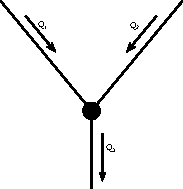
\includegraphics[width=0.30\textwidth]{report/modeling/pictures/interconnections}
\caption{Illustration of an interconnection between two flow inputs and one output.}
\label{fig:interconnections}
\end{figure} 

As any turbulence is neglected, when the two flows join, the flow into pipe three is given as: 
%The two pipes leading into the point are connected, where the wastewater from the two pipes will be added up and transferred to the following pipe. The flow $Q_3$ is calculated as:
\begin{equation} \label{eq:polse_sammenkobling} 
	\boxed{Q_3 = Q_1 + Q_2}
\end{equation} 
%Which is a sum of the flows going into the point. This assumes that there are no turbulence in the joint wastewater from the the pipes. However, this is not the case in a real sewer, but it is deemed sufficient for this model. 
As the concentrate level depends on flow, i.e. $Q \cdot C$, it can be derived by the following equation: 
\begin{equation}\label{eq:polse_concentrat_interconnection}
\begin{array}{l}
	Q_3 \cdot C_3 = Q_1 \cdot C_1 + Q_2 \cdot C_2 \\
	\Updownarrow \\
	C_3 = \frac{C_1 Q_1 + C_2 Q_2}{Q_3}

\end{array}
\end{equation}
%To calculate the concentration in a interconnection the following equation is used: %For the mixing between two flows where one of them is transporting chemicals will be done in similar way as for flows. 
Inserting equation \ref{eq:polse_sammenkobling} into \ref{eq:polse_concentrat_interconnection} the following is obtained for the combined concentrate level of the interconnected pipes.
 
\begin{equation}\label{poop_addition_interconnection}
	\boxed{C_3 = \frac{C_1 \cdot Q_1 + C_2 \cdot Q_2}{Q_1 + Q_2}}
\end{equation}

The two equations for flow and concentrate does not reflect a real interconnection of two flows, but it is assumed to be acceptable on the ground of the assumptions made in section \ref{se:hydraulics_of_sewer_line} and \ref{se:transport_of_concentrate}. 

%Where $C_1$ and $C_2$ are the concentration in the respective pipe $\left[g /m^3 \right]$. \fxnote{Mangler antagelser}   


%This is done to keep the same amount of concentrate within the wastewater, as the algorithm for transporting concentrate depends on flow, as seen in section \ref{se:transport_of_concentrate}. %If it is not calculated like this, thus when the flow is increasing the same will the chemicals within the wastewater, hence it is needed to divided by $Q_3$ to get the right amount of chemicals in the wastewater.  